\chapter{Inverse Synthesis}
\label{chapter:inverse_synth_experiment}

- Goal of this chapter is to perform an inverse synthesis experiment on an FM synthesizer: Dexed, an emulation of the Yamaha DX7 synthesizer. 

To compare the various estimators implemented in SpiegeLib an inverse synthesis experiment was conducted. An additional goal of this experiment is to provide an example of SpiegeLib being used for inverse synthesis. The methodology used for this experiment is modelled after Yee-King et al.'s study on deep learning for automatic synthesizer programming \cite{yee2018automatic}, but with a simplified synthesizer configuration and a unique set of estimators. A VST software emulation of the Yamaha DX7 FM synthesizer was used and six different techniques were compared. In alignment with Vandewalle et al.'s criteria for reproducible research, implementation details, code, and datasets are all available on the \mintinline{python}{spiegelib} online documentation.\footnote{\url{https://spiegelib.github.io/spiegelib/examples/fm_sound_match.html}}

- Breakdown of this chapter: related work section looks at three specific inverse synthesizer experiments and the methods that were 

\section{Related Work}
- Go over the three specific papers that SpiegeLib and the experiments are based on.
- Deep learning: Fully connected and recursive nets: \cite{yee2018automatic}, Convolutional Nets: \cite{barkan2019inversynth}, Genetic Algorithms: \cite{tatar2016automatic}

\subsection{Recurrent Neural Networks}
One of the first works on the application of deep learning to the inverse synthesis problem was published by Matthew Yee-King et al. \cite{yee2018automatic} in 2018. The main contribution of their work was an experiment that showed the effectiveness of a type of recurrent neural networks (RNN) called long short-term memory (LSTM) networks at sound matching on an FM synthesizer audio plugin. RNNs were developed to handle time-series data and receive ordered data which is successively fed into the network architecture. As data is fed into the networks, activation states are stored internally and help to provide temporal context in latter stages of computation. RNNs have been particularly successful for audio generation problems \cite{oord2016wavenet, engel2017neural}. 

Yee-King er al. also experimented with additional machine learning techniques including genetic algorithm (GA), Hill-climber, and  multi-layer perceptron (MLP) methods. They also compared two RNN models: a regular LSTM network as well as a modified LSTM network that had a bi-directional LSTM layer as well as several highway layers, they called this network an LSTM++. Their methodology compared a set of algorithms on a series of successfully more challenging problems on the open-source FM synthesizer Dexed\footnote{\url{https://asb2m10.github.io/dexed/}}. Each problem was focused on programming a subset of the parameters in Dexed; a larger subset was used for each successive problem. A dataset of audio samples paired with the parameters used to generate the audio was created for training each of the deep learning models. Mel-frequency Cepstral Coefficients (MFCCs) were used as input for each of the models. The results were evaluated by looking at the error between MFCCs from target sound and a predicted sound. Results showed that the hill-climber algorithm and the LSTM++ model performed the best. The LSTM++ model showed significant improvements over the other deep learning methods, however the hill-climber performed the best on a majority of the tasks.

Their methodology and software provided a basis for the work presented in the chapter and in the development of SpiegeLib.

\subsection{Convolutional Neural Networks}
Barkan et al. explored convolutional neural networks (CNNs) applied to the inverse synthesis problem in their work which presenting InverSynth \cite{barkan2019deep}. The CNN has been used extensively for image related deep learning tasks and has recently been used successfully in music and audio related tasks including music genre classification \cite{choi2016automatic} and neural audio generation \cite{donahue2018adversarial}. A key feature of CNNs is the use of shared filters that perform convolutions and produce representations at various levels of specificity. The shared filters has allowed them to process large input data such as images and audio with relatively few parameters compared to their fully connected counterparts. 

In their work, Barkan et al. experiment with several different CNN architectures and compare them to a few different fully-connected networks. The focus of their research is performing inverse synthesis on a custom built four oscillator FM synthesizer. They frame the inverse synthesis problem as a classification problem and quantize each of the 23 continuous synthesizer parameters into 16 discrete states. As input they experiment with both STFT as well as raw time-domain audio. Because of the size of these input they created different input representations for the fully-connected networks, for these they used a selection of hand-picked audio features defined in work by Itoyama et al. \cite{itoyama2014parameter}.

Results were evaluated using four different objective methods which evaluate both the ability of the model to match the parameters as well as to reconstruct the target audio. The evaluation metrics used are:
1) Mean Percentile Rank (MPR): ranked position of the correct class measured against predicted classes in the output. Computed independently on each of the 23 synthesizer parameters, each parameter has 16 classes.
2) Top-k Mean Accuracy: measures whether the correct class is among the top-k predicted classes for each parameter.
3) Mean Absolute Error (MAE): this measures the error of the predicted class for each parameter.
4) Spectral Reconstruction Quality: predicted parameters are used to synthesize a predicted audio. The predicted audio is compared against the target audio using error metrics calculated on the STFT and FT representations.

They also conducted a subjective listening experiment which measured the quality of the target audio to the predicted audio for a selection of the methods. Results from the objective and subjective evaluation showed that the depth of the convolutional network played an important role in the quality of the estimator and the best performing networks were two different networks with 6-layers.

\section{Experiment}
\subsection{Synthesizer Configuration}
The first step is defining the synthesizer setup and creating data for training deep learning models. $Dexed$ has 155 parameters controllable through the \mintinline{python}{SynthVST} class. An image of the $Dexed$ interface is shown in figure \ref{fig:dexed}. A subset of nine of these parameters were used in this experiment to turn $Dexed$ into a simple two-oscillator FM synthesizer. A block diagram showing the resulting synth configuration is shown in figure \ref{fig:two_op_fm_block}. In this configuration the second operator modulates the frequency of the first operator. The subset of nine parameters control the amplitude envelope and tuning of the modulating oscillator; this simple synthesizer can produce a wide range of timbres that evolve in various ways over time based on the amplitude envelope of the modulating oscillator. Each operator in $Dexed$ has a complex envelope generator (EG) that can be used to modulate the amplitude of that operator; a diagram and description of the EG is shown in figure \ref{fig:dx7_envelope}. The complex envelope generator has five independent stages that are controlled by a set of parameters that control the length and amplitude of each stage. For this experiment only the EG for the second operator had parameters for estimation: $LEVEL 2-4$ and $RATE 2-4$. The $RATE 1$ and $LEVEL 1$ parameters were locked to the minmimum rate and highest level, effectively turning off the initial rise portion of the envelope. Three parameters controlling the pitch and tuning of the second operator were also open for estimation. All parameters have a normalized range from $[0-1]$. The remainder of the available parameters in $Dexed$ are locked at values to create a simple sine wave generator that is being frequency modulated by the second operator. The \mintinline{python}{SynthVST} class provides methods for overriding and freezing parameters as well as saving and loading parameter settings as JSON files. 

\begin{figure}[ht]
    \centering
    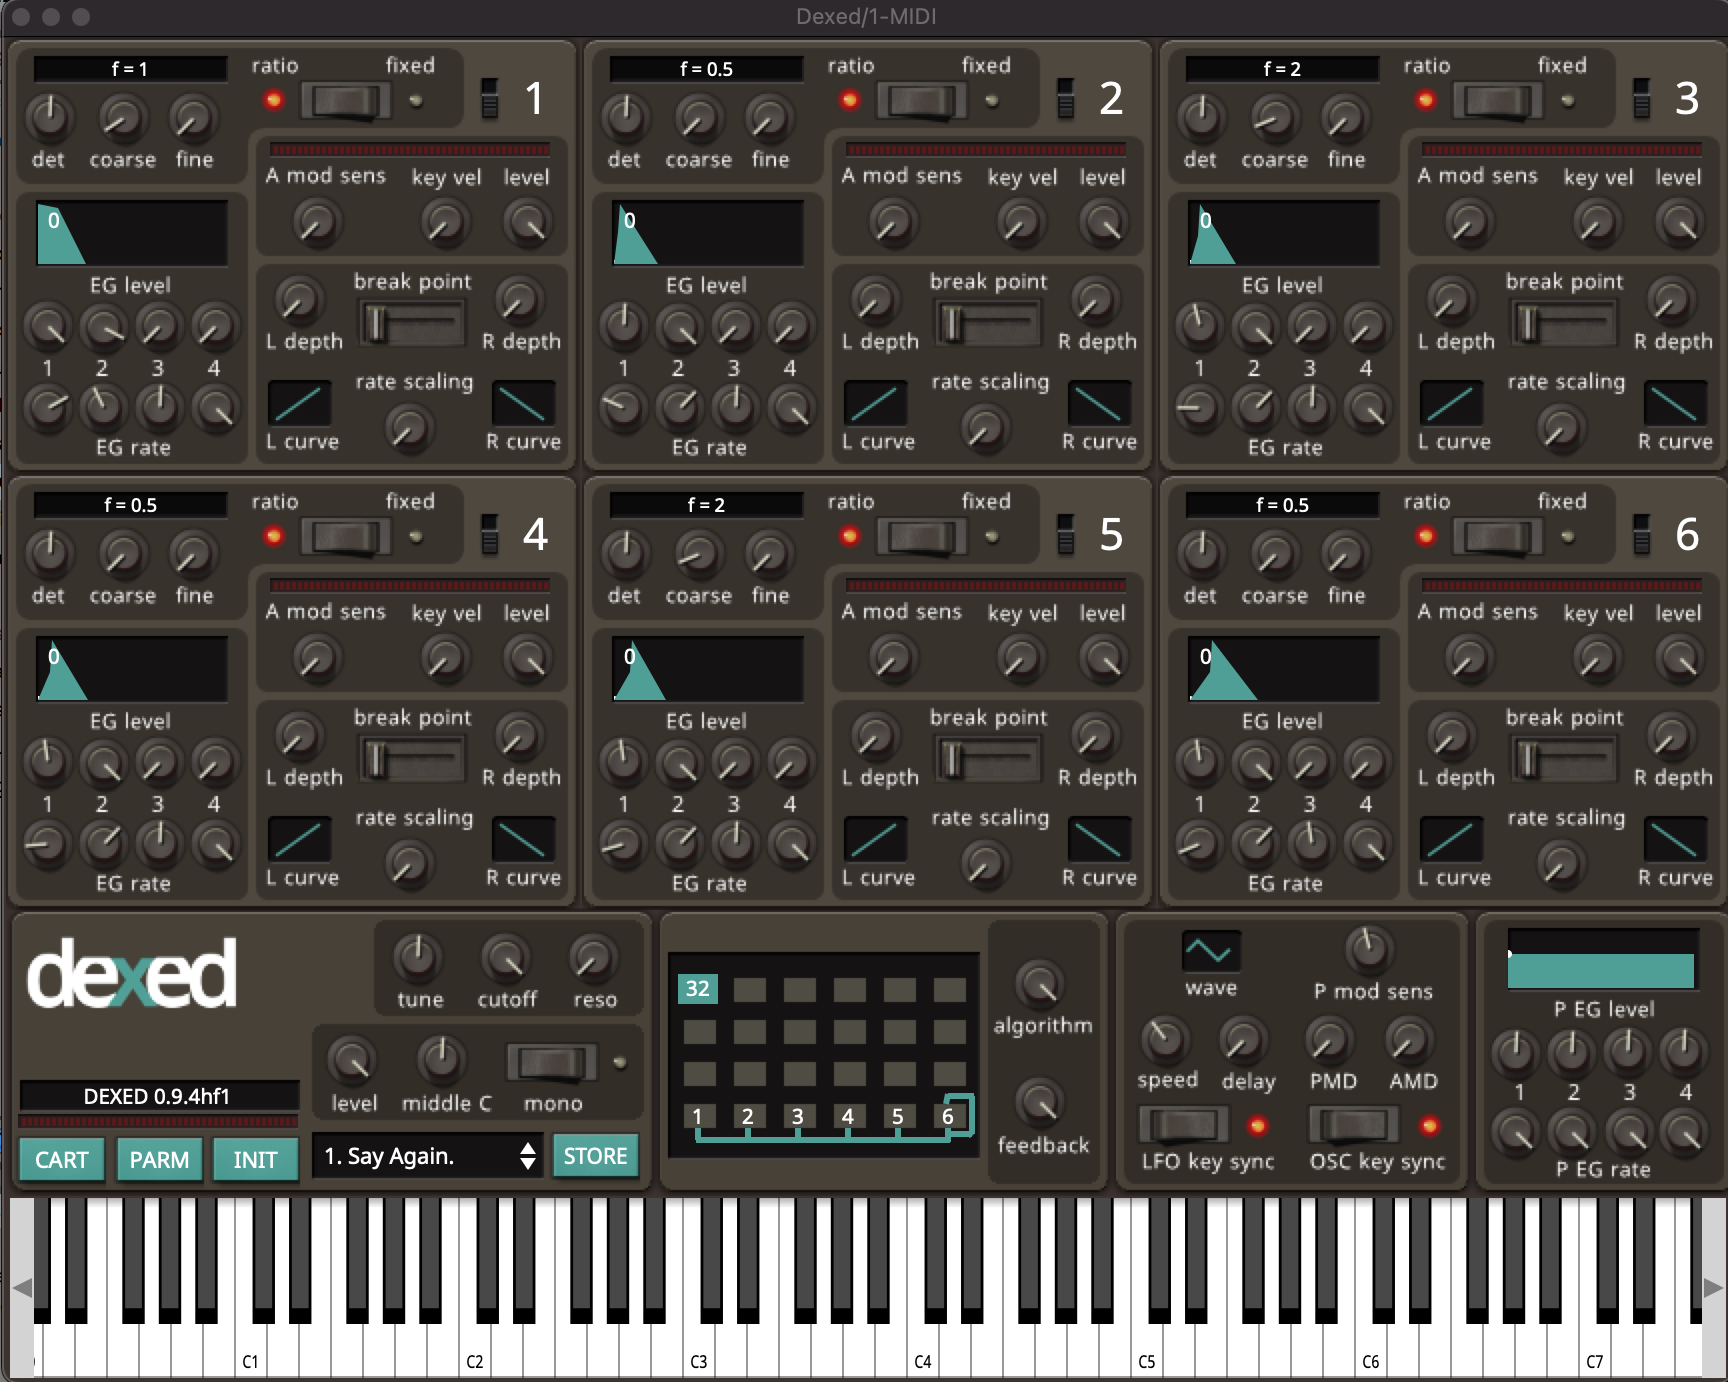
\includegraphics[width=0.75\textwidth]{figures/spiegelib/dexed.png}
    \caption{The Dexed synthesizer interface. Dexed is an open-source emulation of the Yamaha DX7 FM synthesizer and it was used in the experiments in this chapter/}
    \label{fig:dexed}
\end{figure}

\begin{figure}[ht]
    \centering
    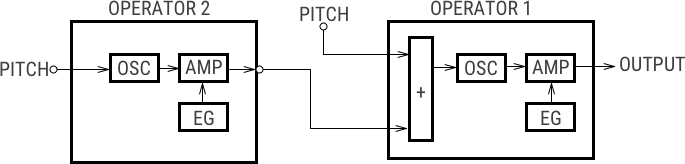
\includegraphics[width=0.9\textwidth]{figures/spiegelib/two_op_fm_block.png}
    \caption{Block diagram of a two operator FM synthesizer. Dexed has six independent operators that can be configured in various ways, however for the experiments conducted here only the first two operators were used and were setup in this configuration.}
    \label{fig:two_op_fm_block}
\end{figure}

\begin{figure}[ht]
    \centering
    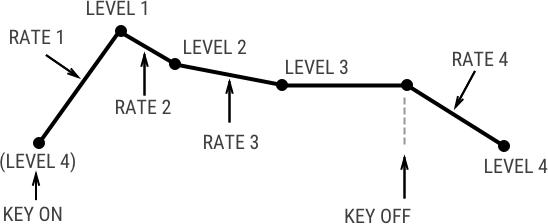
\includegraphics[width=0.75\textwidth]{figures/spiegelib/Yamaha DX7 Envelope.png}
    \caption{Diagram of an envelope generator in the Yamaha DX7 and Dexed. The envelope has five independent stages. During the first three stages the envelope moves linearly from level 4 to level 1, then to level 2, then to level 3. Each of these levels is controllable and the length of time taken to move to each level is also definable. This movement is triggered by a key-on event. Once the envelope has progressed to level 3 it stays at that level until a key-off event is received, at which point the envelope progresses back to level 4.}
    \label{fig:dx7_envelope}
\end{figure}

% \begin{table}[]
%     \centering
%     \begin{tabular}{c|c}
%          &  \\
%          & 
%     \end{tabular}
%     \caption{Caption}
%     \label{tab:my_label}
% \end{table}

\subsection{Dataset}
The \mintinline{python}{DatasetGenerator} class was then used to create datasets for deep learning training. All deep learning models, except for the CNN, used a 13-band MFCC calculated with a frame size of 2048 samples and a hop size of 1024 samples. The input of the CNN was the magnitude spectrum from a STFT, calculated using an FFT with 512 bins and a hop size of 256 samples. Using an instance of \mintinline{python}{DatasetGenerator}, 50,000 training examples and 10,000 validation examples were generated by randomly sampling the nine parameters from $Dexed$. Resulting feature vectors were normalized by removing the mean and scaling to unit variance using methods within the \mintinline{python}{FeatureBase} base class. Datasets and settings for normalization were then stored as NumPy files for later use.

\subsection{Estimation Techniques}
List out all the techniques used in the experiment.

\subsection{Models}
All deep learning models are defined in classes within \mintinline{python}{spiegelib} and all inherit from \mintinline{python}{TFEstimatorBase}. Three models derived from work by Yee-King et al. \cite{yee2018automatic} were used: 1) A simple multi-layer perceptron with three hidden layers, all with a ReLu activation, 2) a LSTM recurrent network with three layers and dense output, and 3) a LSTM++ networks which contains a single bidirectional LSTM node followed by a dense layer with an elu activation, six highway layers, and a dense output. One convolutional neural network (CNN) derived from work by Barkan et al. \cite{barkan2019inversynth} was also included: this network featured six layers of strided convolutions followed by a dropout layer and a dense output. Specific details of all these models is provided in appendx \ref{appendix:spiegelib_models}.

Models were trained using an $Adam$ optimizer \cite{kingma2014adam} with a learning rate of 0.001, batch sizes of 64, and used an early stopping callback which halted training if validation loss was stagnant for 10 epochs to prevent overfitting. Ideally the loss function would be computed directly on audio rendered from $Dexed$ using the predicted parameters, but that is challenging to implement, so the loss is computed on the parameter values which has been standard in previous work \cite{yee2018automatic, barkan2019inversynth}.

The loss function used was the RMS error between the target parameter values and the predicted parameter values, which is given by the following formula where $N$ is the number parameters, $y$ is the true parameter values, and $\hat{y}$ is the predicted parameter values:

\begin{equation}
    \ell(y, \hat{y}) = \sqrt{\frac{\sum_{i \in N}{(y_i - \hat{y_i})^2}}{N}} 
\end{equation}

Logging of training and validation progress was recorded using the \mintinline{python}{TFEpochLogger} class. Plots of training and validation accuracy and loss for the LSTM++ model are shown in figure \ref{fig:lstm_bi_train}. 

% TODO: add in some of the other loss plots (probably all of them) and remark on the differences betwee them.

Trained models are then saved for future use.

\begin{figure}[ht]
\begin{center}
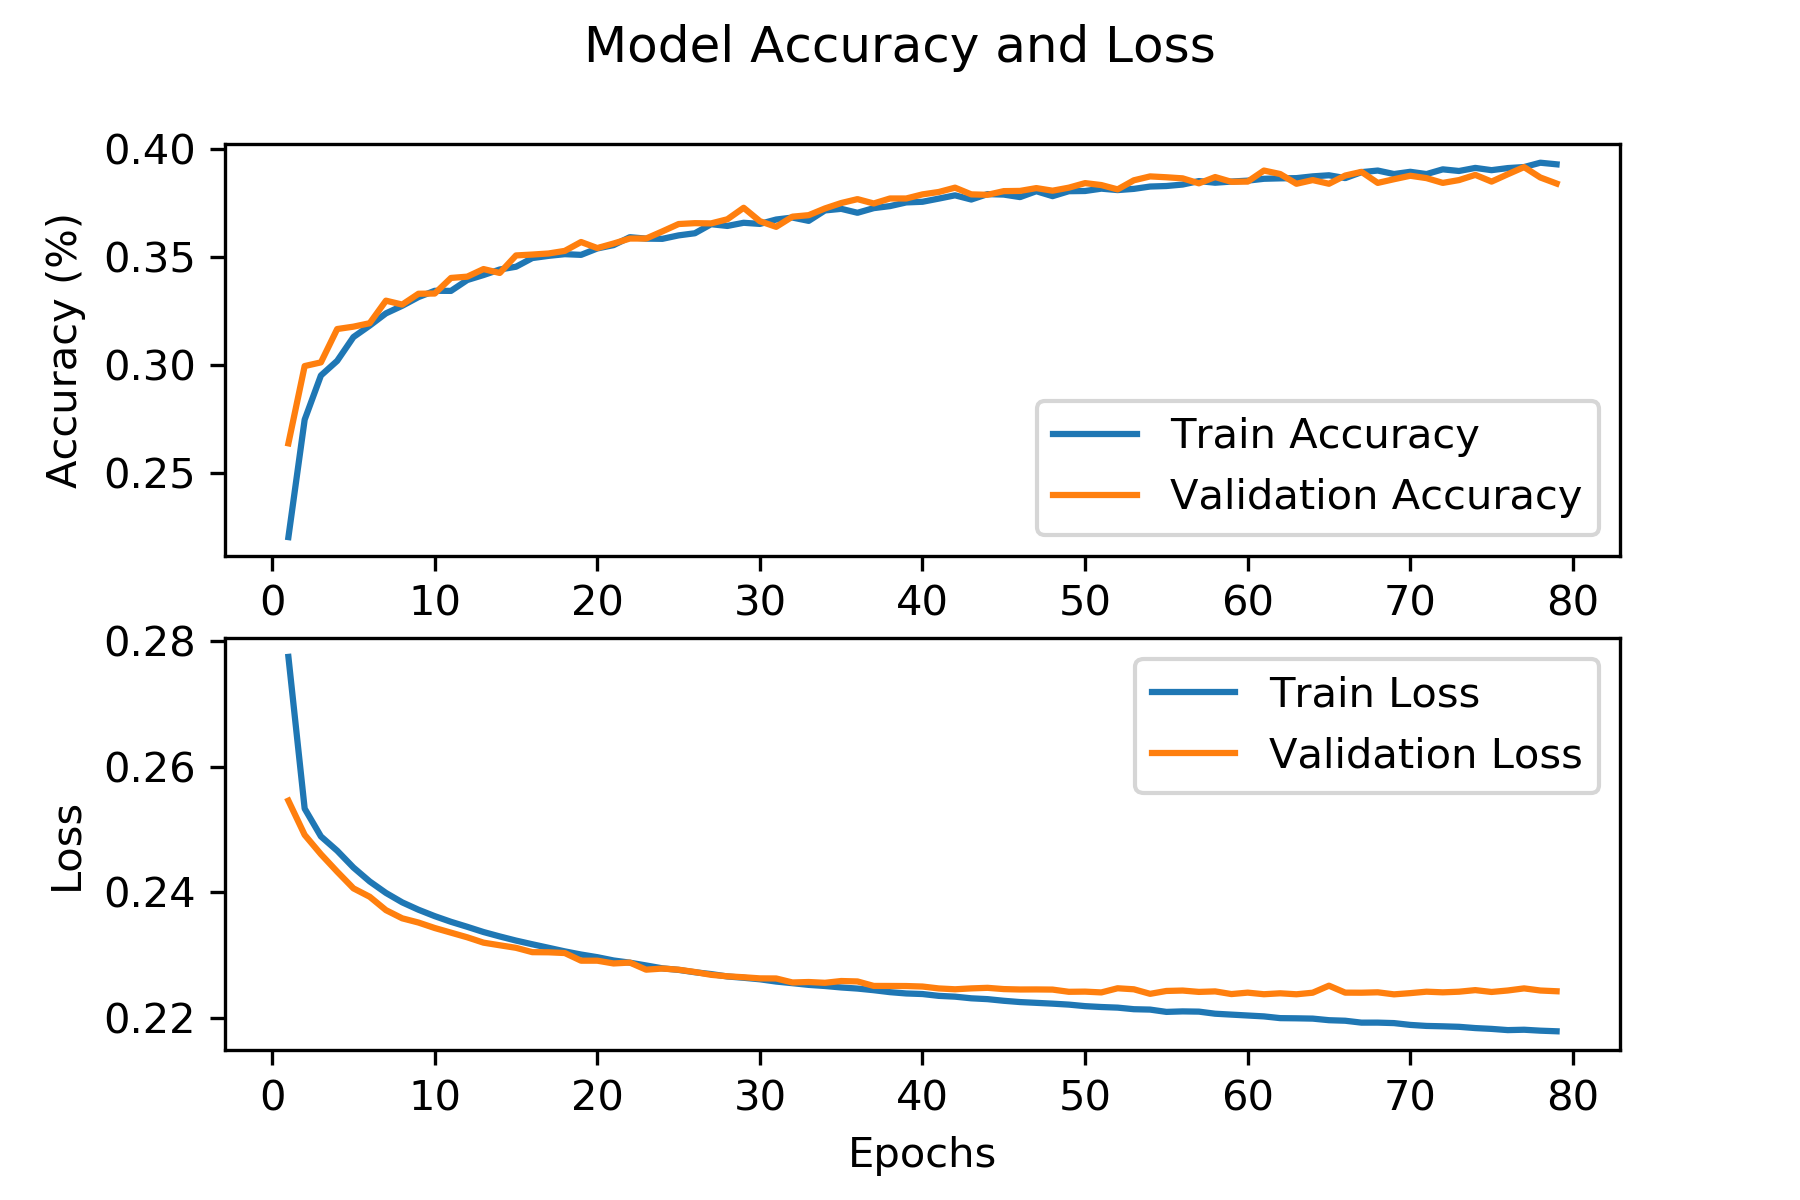
\includegraphics[width=0.75\columnwidth]{blstm_training.png}
\caption{Traing and validation accuracy and loss over epochs for LSTM++ model training.}
\label{fig:lstm_bi_train}
\end{center}
\end{figure}

\subsection{Genetic Algorithms}
Two different GAs were used: a basic single-objective GA and a multi-objective NSGA III. The multi-ojective GA was derived from work conducted by \cite{macret2012automatic} that used the algorithm to automatically tune the parameters of a Teenage Engineering OP-1\footnote{\url{https://teenage.engineering/products/op-1}} synthesizer. In the GAs the $fitness$ (which is equivalent to the loss in deep learning) is easily computed directly on the audio rendered from $Dexed$. In the case of the basic GA the $fitness$ is computed as the mean absolute error (MAE) between 13-band MFCCs from the target and the individual. Three different metrics were used for evaluating the $fitness$ of an individual for the NSGA-III algorithm, MAE between: 1) a 13-band MFCC, 2) magnitude spectrum from an FFT, and 3) five spectral features. MAE is given by the following formula, where $N$ is the number of features, $y$ is the target, and $\hat{y}$ is the predicted individual:

\begin{equation}
    \text{MAE} = \frac{\sum_{i \in N}{|y_i - \hat{y}_i|}}{N}
\end{equation}

Both genetic algorithms were run for 100 generations for each sound target. The basic GA and NSGA used population sizes of 300 and 100 individuals respectively. Figure \ref{fig:nsga_fitness} shows the minimum spectral error achieved by an individual during each iteration of the NSGA algorithm on one of the target sounds. The plot shows a period of rapid improvement during early iterations, with some short periods of stagnation, followed by longer periods where the algorithm is unable to find an individual that is an improvement over those in the current population.

% TODO: Add in the other population generation plots for each objective

\begin{figure}[ht]
\begin{center}
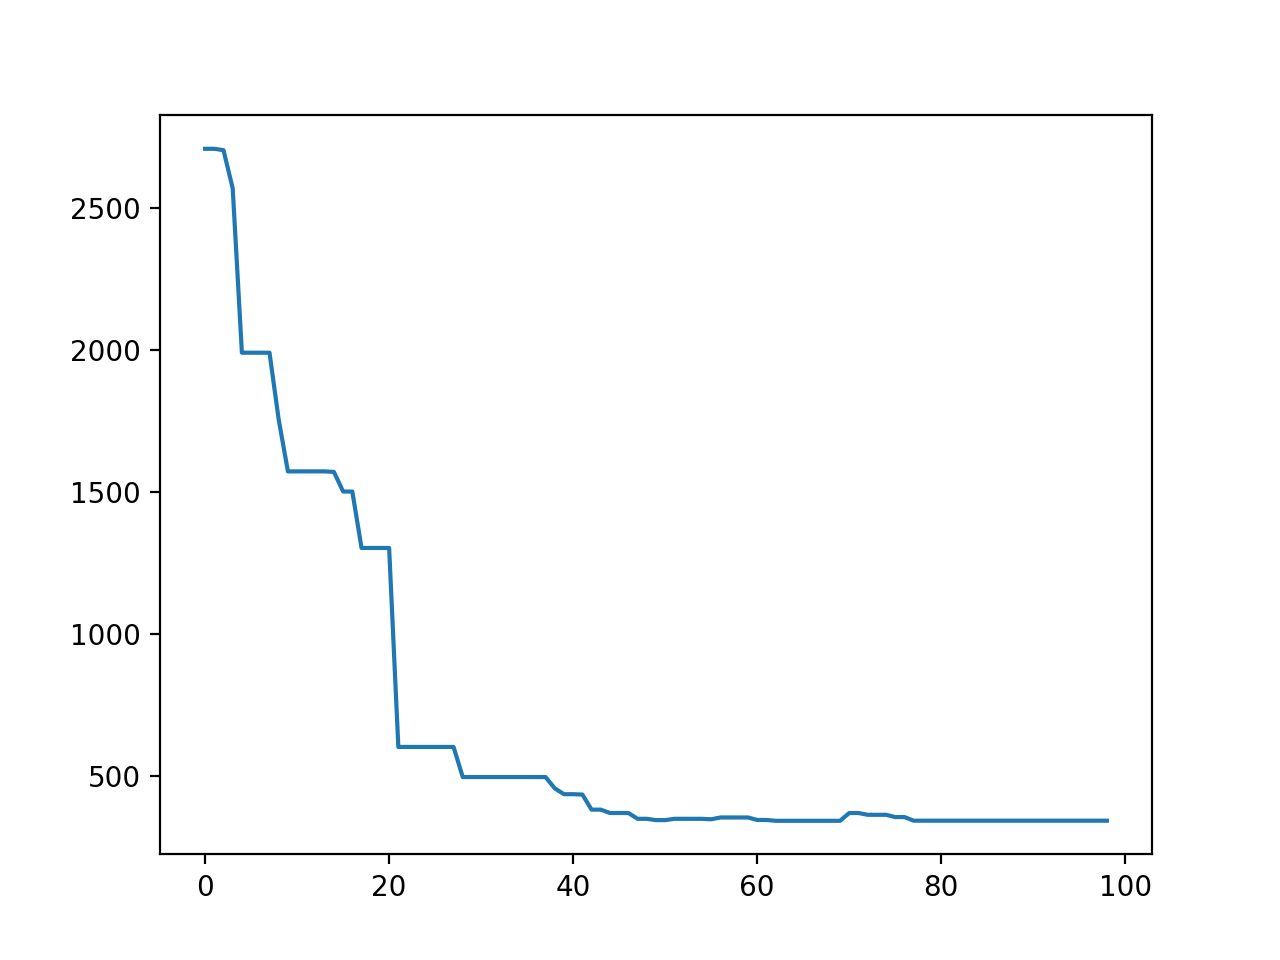
\includegraphics[width=0.7\columnwidth]{nsga_target_15_FFT.png}
\caption{Minimum FFT MAE in the population at each generation to target sound 15 for NSGA III estimator.}
\label{fig:nsga_fitness}
\end{center}
\end{figure}

\section{Evaluation}
To evaluate each of the techniques an evaluation dataset containing 25 random sounds generated using the same nine-parameter $Dexed$ configuration was used. Using the sounds generated using the same synthesizer configuration means that an error of zero is possible, which provides a stable baseline for comparing each of the methods. All estimators were run on each one of the 25 target sounds using the \mintinline{python}{SoundMatch} class. This resulted in a set of audio files generated from $Dexed$ using the estimated parameters from each estimator run on each of the 25 target sounds. All of the resulting sounds are available for listening online on the SpiegeLib docs page\footnote{\url{https://spiegelib.github.io/spiegelib/examples/fm_sound_match_pages/fm_sound_match_listen.html}}. Quantitative and qualitative evaluation was conducted on these sounds.

\subsection{Quantitative Evaluation}
Evaluation was conducted by comparing the predicted audio files to the target audio using MAE computed on MFCCs, which is the same method that was used during evaluation by Yee-King et al. \cite{yee2018automatic}. Results for mean absolute error (MAE) which have been summarized using mean, standard deviation, minimum, and maximum, are shown for each estimator in table \ref{tbl:sound_match_eval}. Both GAs performed better than the deep learning approaches with the NSGA III having the best overall score. For deep learning approaches, the LSTM++ model achieved the best mean score.

\begin{table}[t]
\centering
\caption{Results from sound matching evaluation}
\label{tbl:sound_match_eval}
\begin{threeparttable}
\begin{tabular}{l|cccc}
\toprule
$Method$ & $Mean$ & $SD$ & $Min$ & $Max$ \\
\midrule
$MLP$ & 8.55 & 6.77 & 1.92 & 34.12 \\
$CNN$ & 7.88 & 4.26 & 2.68 & 20.89 \\
$LSTM$ & 6.12 & 3.76 & 1.20 & 19.36 \\
$LSTM++$ & 4.91 & 6.50 & 2.12 & 21.51 \\
$GA$ & 2.25 & 2.58 & 0.70 & 11.17 \\
$NSGA III$ & \textbf{0.81} & \textbf{0.89} & \textbf{0.001} & \textbf{3.06} \\
\bottomrule
\end{tabular}
\begin{tablenotes}[para, flushleft]
\footnotesize
\item Values shown are calculated from the mean absolute error (MAE) calculated during MFCC evaluation. Smaller MAE values indicate more similar matches. The NSGA III estimator received the best scores, which are shown in bold font.
\end{tablenotes}
\end{threeparttable}
%\vspace{5mm}
\end{table}

% TODO informal listening based on MAE so I can comment on the results in terms of MAE

Histograms of the the MAE were also plotted for each estimator using the \mintinline{python}{plot_hist()} method in \mintinline{python}{EvaluationBase}. Histograms of the MAE for all predictions made by all estimators are shown in figure \ref{fig:group_hist}. These plots clearly show the NSGA III as the winner in terms of MFCC MAE; 24/25 of the predicted sounds have an MAE less than 2.5 (the smallest histogram bin), and the other sound is still less than 5. For the deep learning models, the LSTM++ performed the best overall, however the LSTM model produced more results that had a MAE less than 2.5. The MLP model performed the worst overall and the histogram shows a wide range of results, the MLP also produced a result with the worst individual score of 34.12. The CNN model performed only slightly better than the MLP and had no predictions with a score less than 2.5.

\begin{table}[t]
\centering
\caption{Results from sound matching evaluation}
\label{tbl:param_eval_eg}
\begin{tabular}{r|ccc|ccc|c}
\toprule
{} & \multicolumn{3}{c}{EG RATE} & \multicolumn{3}{c}{EG LEVEL} & {} \\
{} & 2 & 3 & 4 & 2 & 3 & 4 & Mean \\
\midrule
MLP      &     0.0011 &     0.0902 &     0.0223 &      0.0096 &      0.0134 &      0.0215 &   0.0264 \\
LSTM     &     0.0002 &     \textbf{0.0081} &     0.0191 &      0.0042 &      0.0020 &      0.0331 &   0.0111 \\
5-LSTM++ &     0.0007 &     0.0354 &     0.0210 &      0.0069 &      0.0037 &      0.0348 &   0.0171 \\
LSTM++   &     \textbf{0.0002} &     0.0241 &     0.0306 &      0.0072 &      0.0025 &      0.0434 &   0.0180 \\
Conv6    &     0.0022 &     0.0212 &     0.0583 &      0.0024 &      0.0071 &      0.0223 &   0.0189 \\
Conv6s   &     0.0008 &     0.0252 &     0.0280 &      0.0107 &      0.0029 &      0.0307 &   0.0164 \\
Conv5    &     0.0026 &     0.0230 &     0.0300 &      0.0055 &      0.0108 &      0.0321 &   0.0174 \\
Conv5s   &     0.0012 &     0.0293 &     0.0111 &      0.0067 &      0.0033 &      0.0228 &   0.0124 \\
\midrule
Mean  &     0.0011 &     0.0321 &     0.0275 &      0.0067 &      0.0057 &      0.0301 &   0.0172 \\
\bottomrule
\end{tabular}
\end{table}

\begin{table}[t]
\centering
\caption{Results from sound matching evaluation}
\label{tbl:param_eval_osc}
\begin{tabular}{r|ccc|c}
\toprule
{} & \multicolumn{3}{c}{OSC} & {} \\
{} & Coarse & Fine & Detune & Mean \\
\midrule
MLP      &    0.0053 &  0.0958 &      0.0709 & 0.0573 \\
LSTM     &    0.0044 &  0.0770 &      0.0606 & 0.0473 \\
5-LSTM++ &    0.0056 &  0.0696 &      0.0711 & 0.0488 \\
LSTM++   &    0.0052 &  0.0933 &      0.0723 & 0.0570 \\
Conv6    &    0.0051 &  0.0852 &      0.0681 & 0.0528 \\
Conv6s   &    0.0063 &  0.0916 &      0.0651 & 0.0543 \\
Conv5    &    0.0093 &  0.0698 &      0.0721 & 0.0504 \\
Conv5s   &    0.0068 &  0.0729 &      0.0704 & 0.0500 \\
\midrule
Mean     &    0.0060 &  0.0819 &      0.0689 & 0.0523 \\
\bottomrule
\end{tabular}
\end{table}
% TODO objective evaluation based on the parameter values?

\subsection{Qualitative Evaluation}
Spectrograms of one target sound and predictions made by each of the estimators for that target are shown in figure \ref{fig:group_spect}. The selected example was one of the most challenging targets; both the GAs, the LSTM, and the MLP received their worst individual score on it. The most clear difference between the spectrograms can be seen in the temporal evaluation of the harmonics, which is caused by the EG applied to the amplitude of the second operator. In the target the envelope has two obvious components: 1) gradually descending over the first half, and then 2) remaining constant for the remainder of the sound. All the predictions have a similar shape, however only the NSGA III is able to match the shape of of those two sections of the envelope. The MLP, which performed the worst, has two envelope sections, but the first section descends too radpidly and then the constant section is at the incorrect amplitude.

Another aspect of the spectrograms that can be identified are periodic amplitude modulations occuring along the horizontal axis of the harmonics. These show up as period dark notches on the harmonic. These spacing between the horizontal notches indicates the tuning of the second operator that is modulating the frequency of the first operator. In the target this modulation pattern shows up in the first half of the clip, but not the second. Only the NSGA III was able to correctly match the tuning in both sections of the audio. 

% Did I mess up the charts for the CNN and the GA?? Those shouldn't be different I don't think?

\begin{figure}[t]
\begin{center}
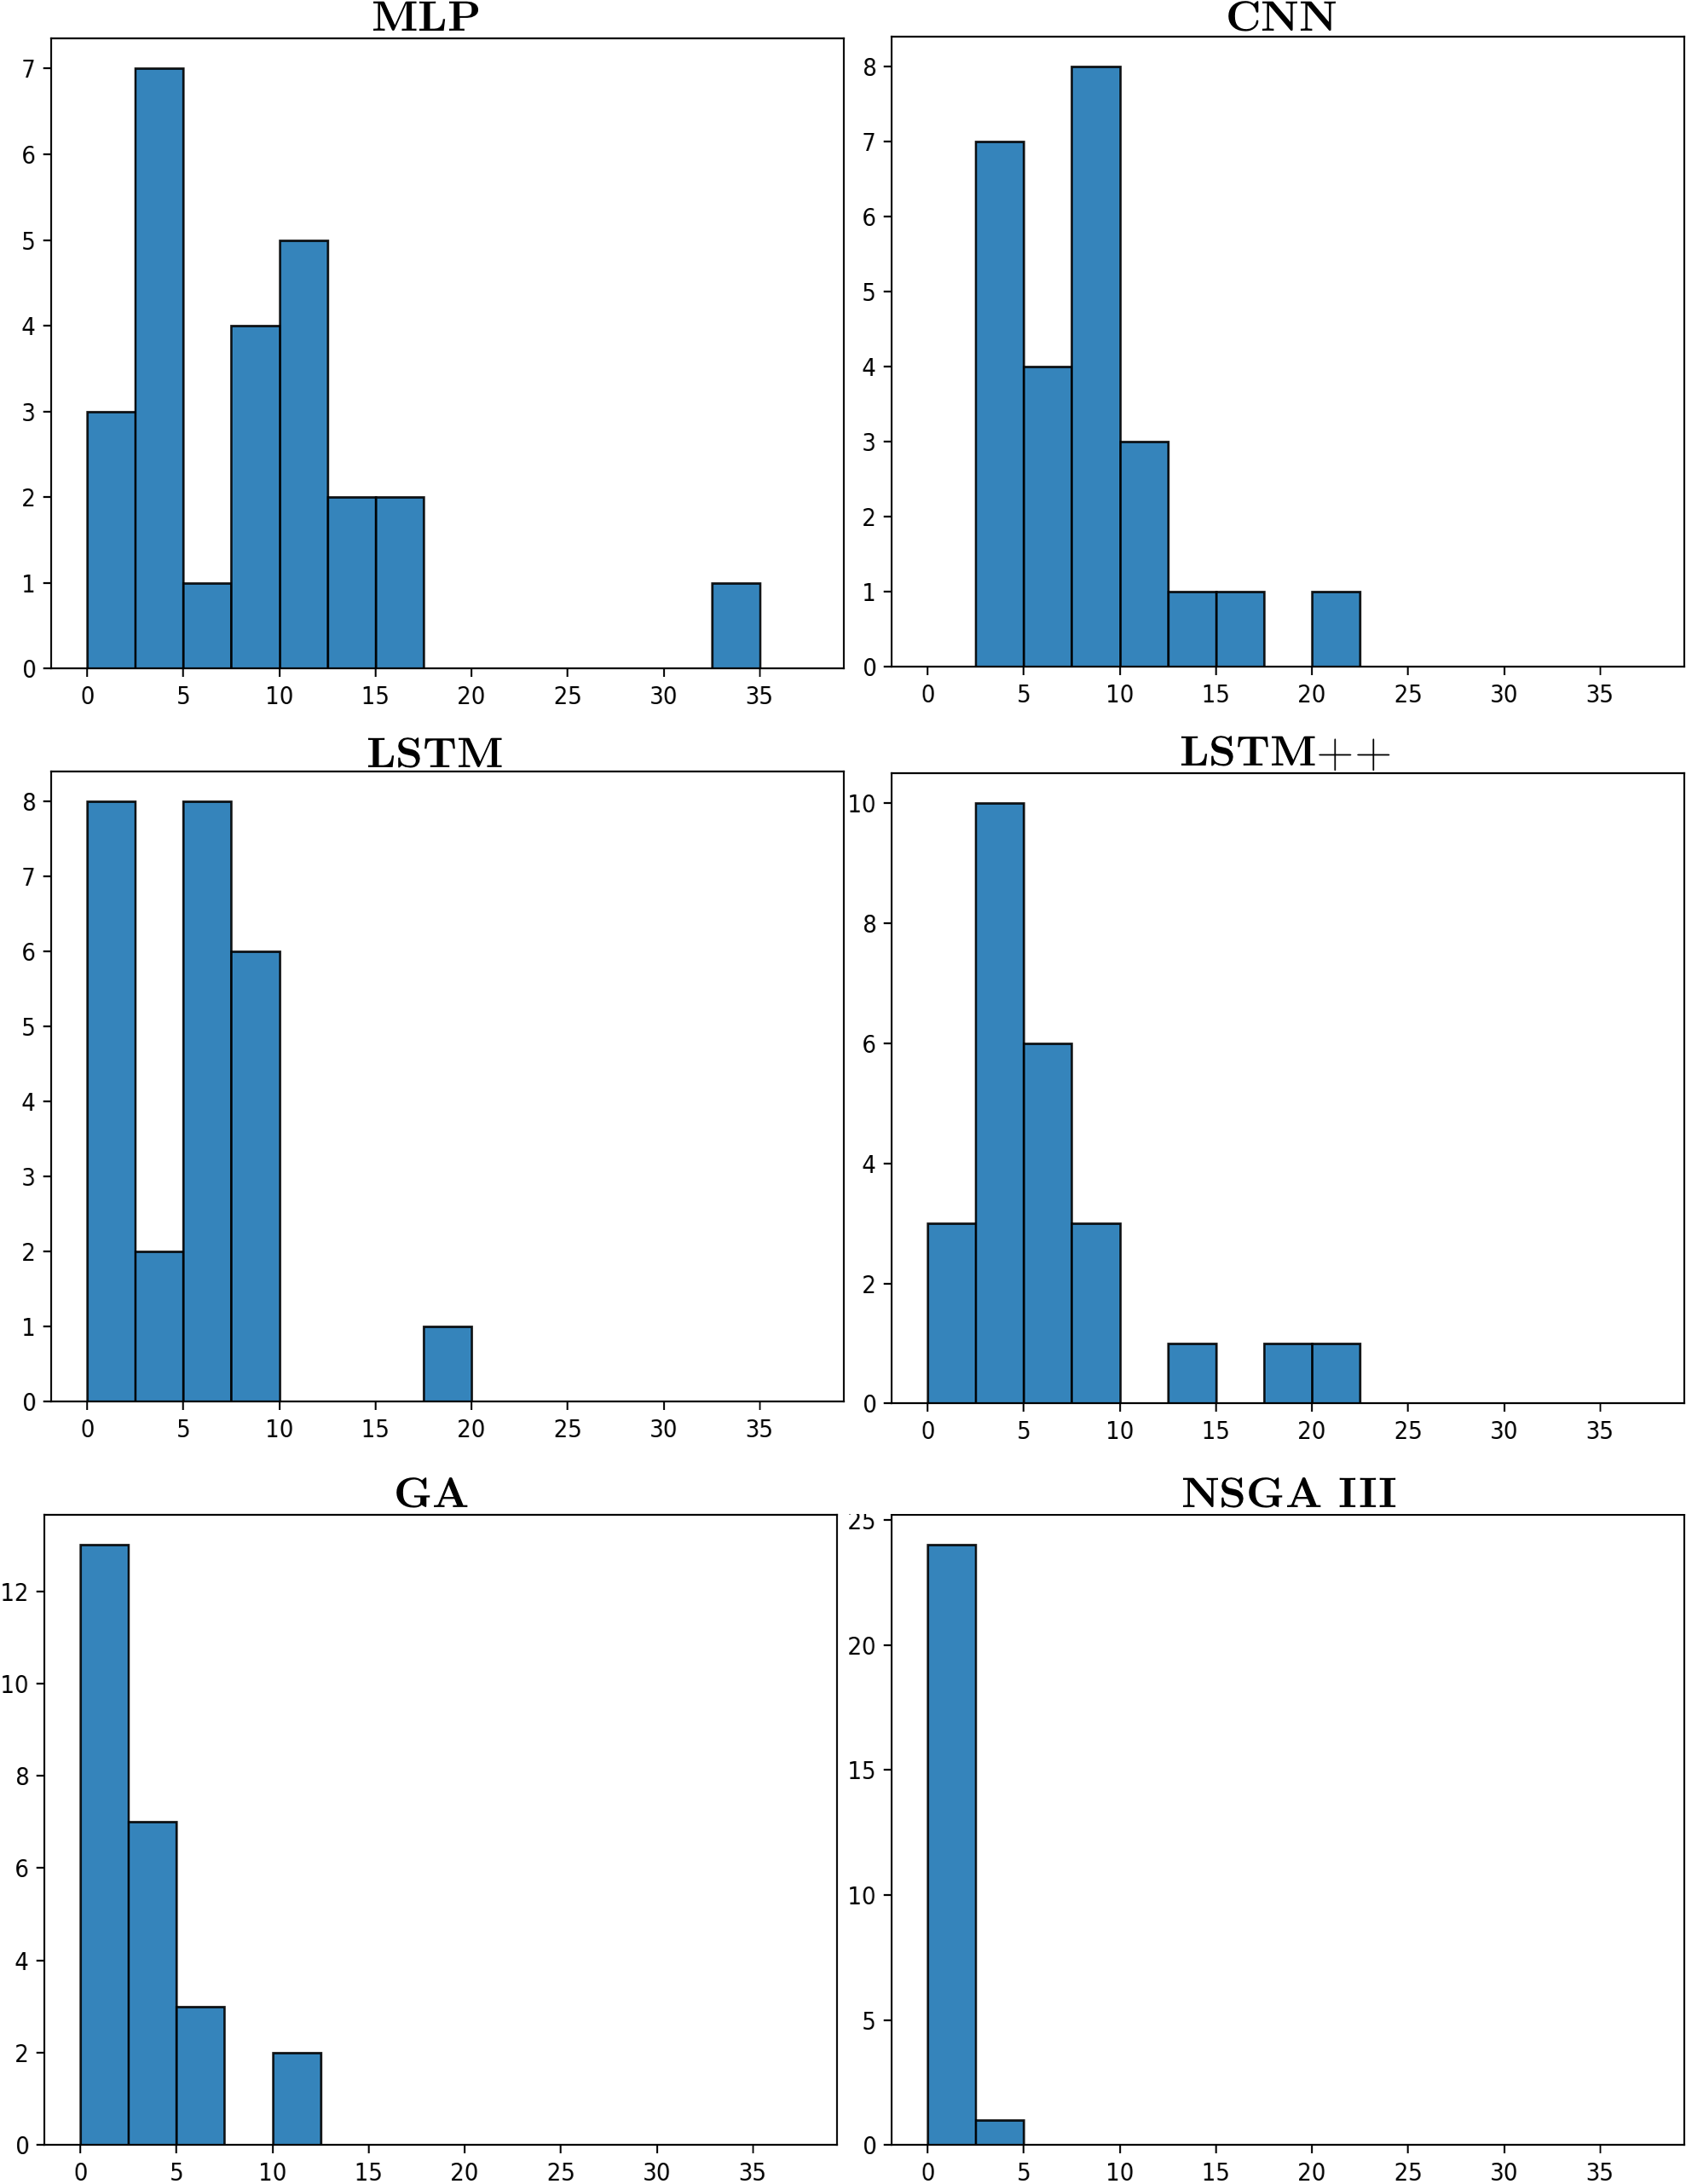
\includegraphics[width=0.75\textwidth]{hist_group_v3.png}
\caption{Histogram shows the MAE values resulting from MFCC evaluation run on a set of 25 sound targets for all estimators. Lower MAE values indicate a closer sound match.}
\label{fig:group_hist}
\end{center}
\end{figure}

\begin{figure}[t]
\begin{center}
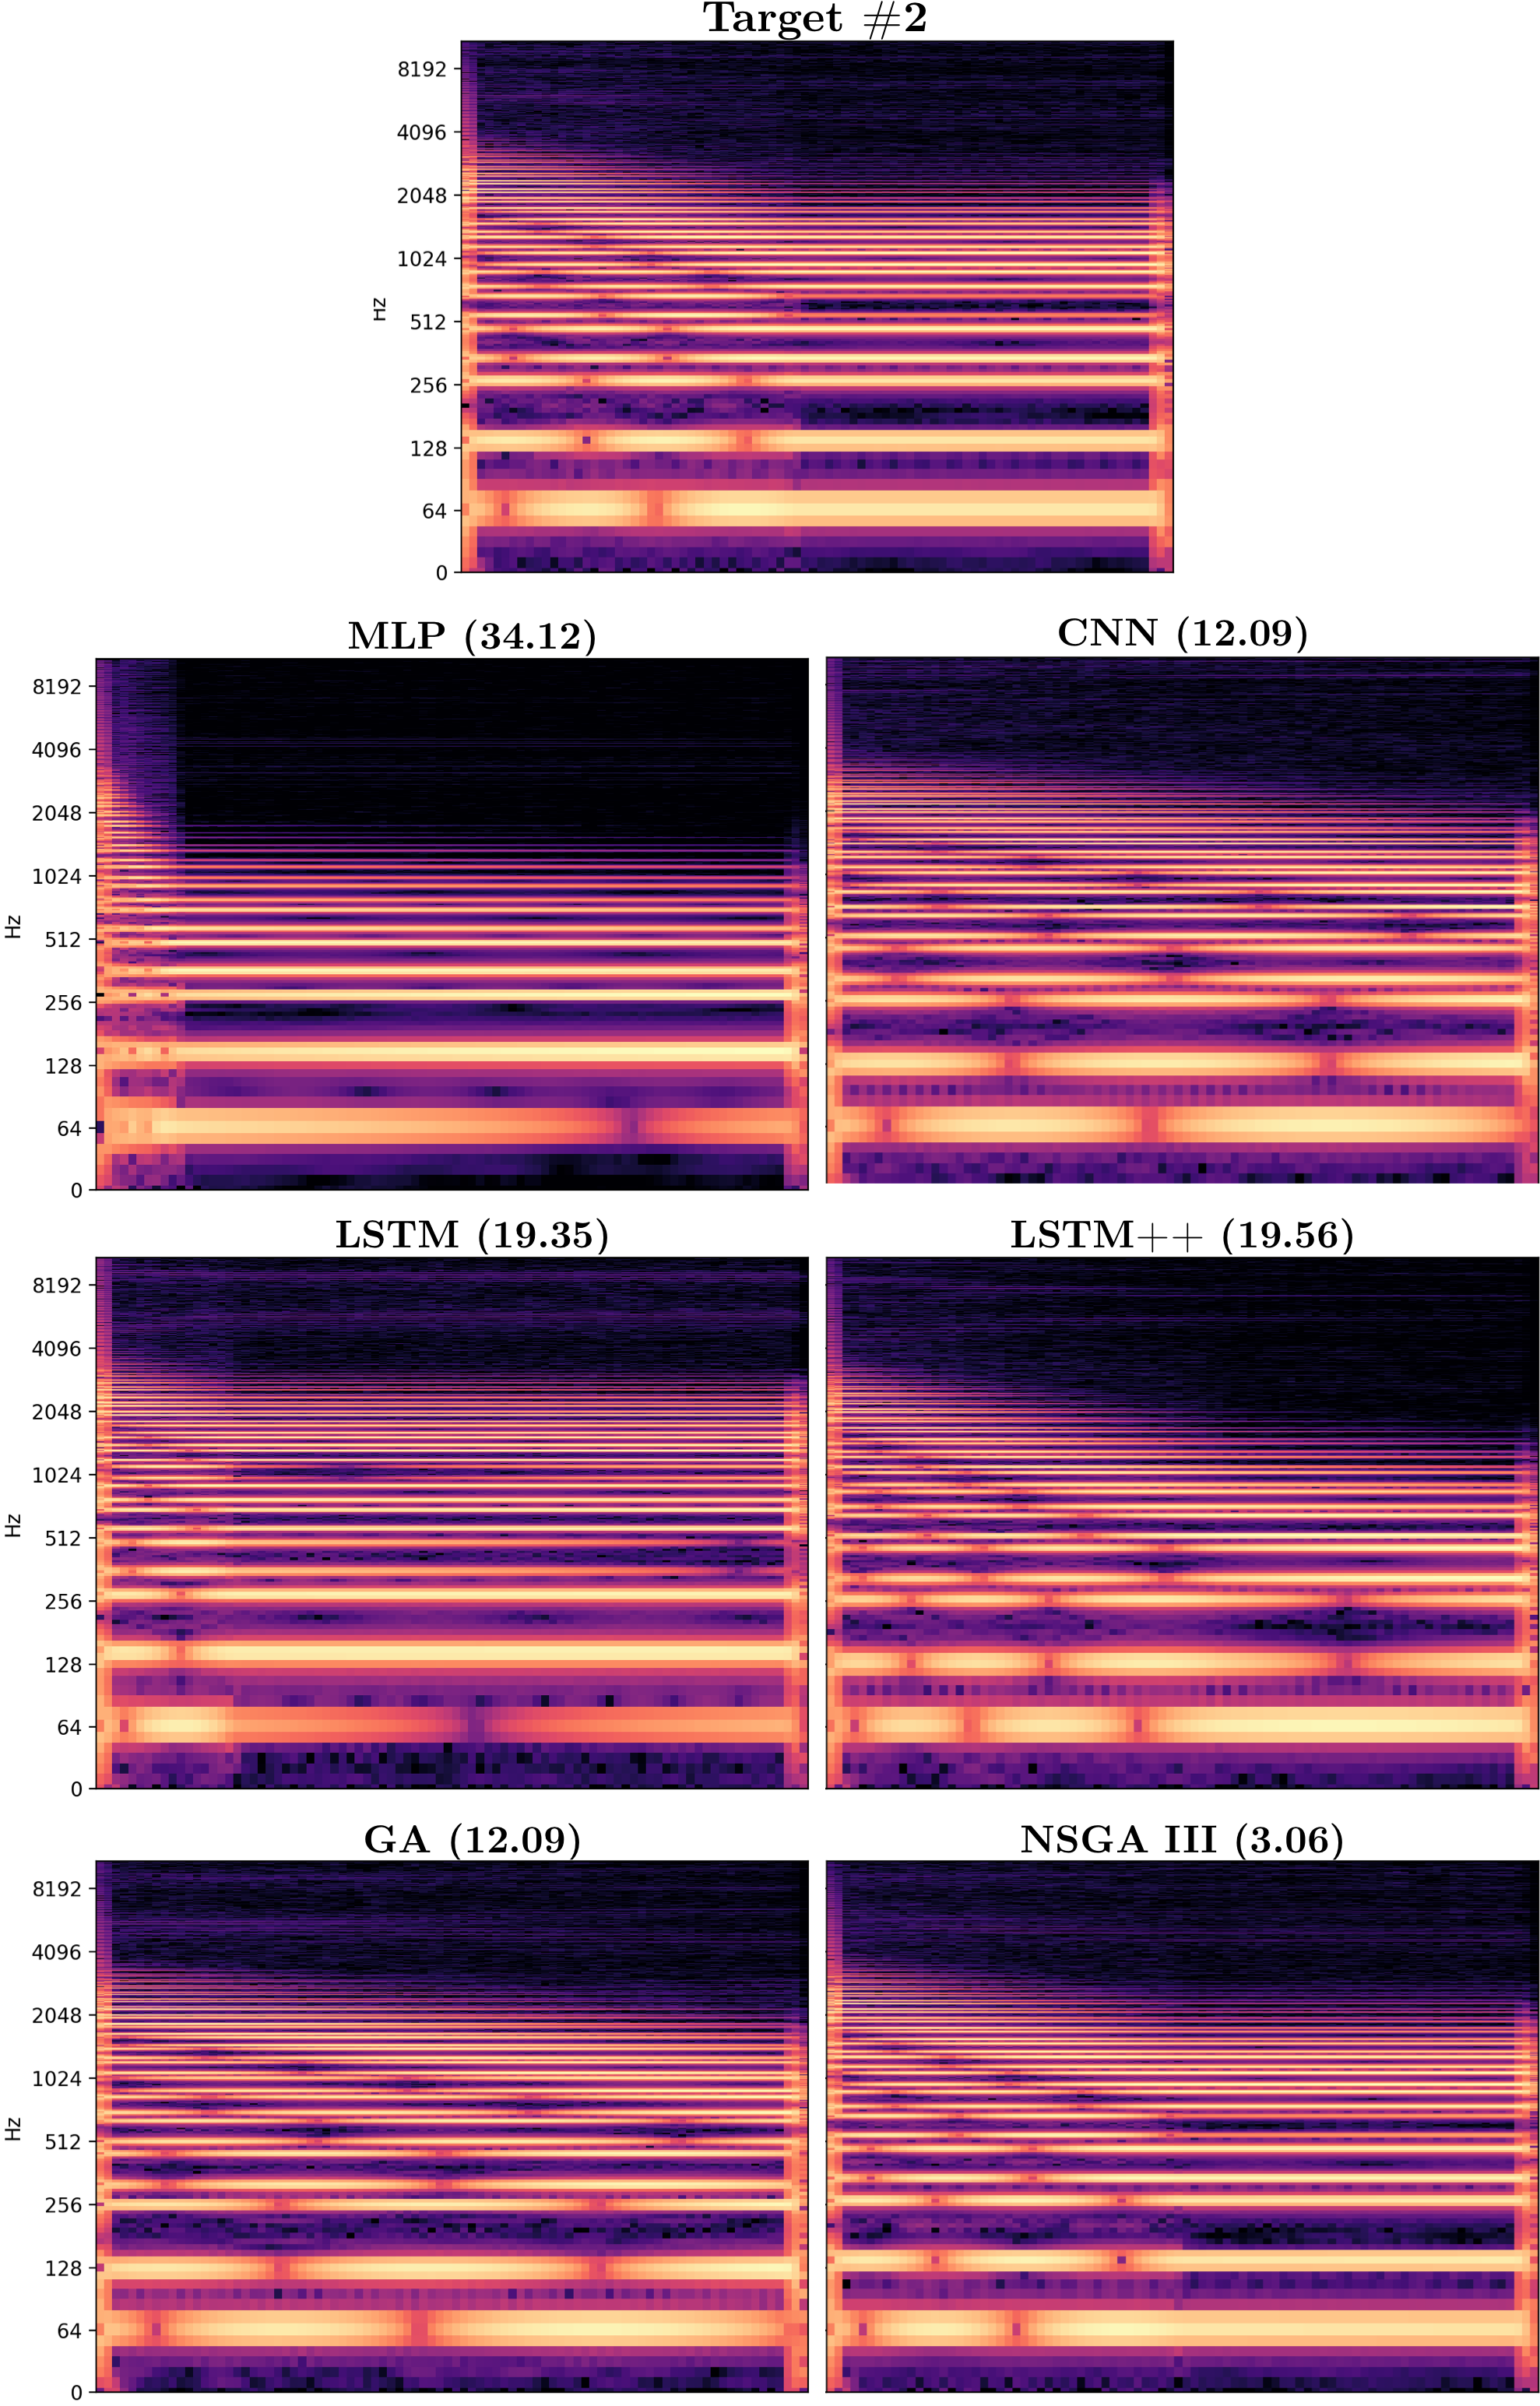
\includegraphics[width=0.75\textwidth]{spect_group_v1.png}
\caption{Spectrogram plots of a target sound and sound match predictions made by each estimator. The value next to the estimator name is the MAE value from MFCC evaluation for that prediction (lower MAE values indicate a closer match).}
\label{fig:group_spect}
\end{center}
\end{figure}

% I think this can be removed?
% To evaluate to the resulting predictions the \mintinline{python}{MFCCEval} class was used, which calculates error and distance metrics on MFCCs of a target and prediction. Results for mean absolute error (MAE) which have been summarized using mean, standard deviation, minimum, and maximum, are shown for each estimator in table \ref{tbl:sound_match_eval}. Both GAs performed better than the deep learning approaches with the NSGA III having the best overall score. For deep learning approaches, the LSTM++ model achieved the best mean score. Histograms of the the MAE were also plotted for each estimator using the \mintinline{python}{plot_hist()} method in \mintinline{python}{EvaluationBase}. Histograms of the MAE for all predictions made by all estimators are shown in figure \ref{fig:group_hist}. Spectrograms of one target sound and sound match predictions made by each of the estimators for that target are shown in figure \ref{fig:group_spect}. For this particular target, spectrograms reveal that while the frequency and distribution of the harmonics was relatively close for each estimation, all estimators except for the NSGA III struggled with matching the temporal envelope of the spectrum.

\section{Conclusion}

- Conducted an inverse synthesis experiment on a VST software synthesizer Dexed
- Results showed that the GAs performed the best via objective evaluation
- LSTM++ model performed the best out of the deep learning models
- Comparison of the search versus modelling methods for inverse synthesis
- Discussion of the parameter sampling methods -- uniform sampling may not provide the best method for training the deep learning models to learn sounds that a human might program
- Challenges associated with programming a VST software synth